\documentclass{article}

\usepackage{aligned-overset}
\usepackage{amsmath}
\usepackage{amssymb}
\usepackage{bbm}
\usepackage[shortlabels]{enumitem}
\usepackage{genealogytree}
\usepackage{hyperref}
\usepackage[utf8]{inputenc}
\usepackage{interval}
\intervalconfig{
  soft open fences
}

\usepackage{makecell}
\usepackage{mathtools}
\usepackage{physics}
\usepackage{tabularx}
\usepackage{tikz}
\usetikzlibrary{positioning}
\usepackage{xcolor}
\definecolor{light-gray}{gray}{.9}

\author{Karsten Lehmann}
\date{WiSe 2020}
\title{Mitschriften Algorithmen und Datenstrukturen}

\begin{document}


\maketitle
\newpage

\section*{Vom Problem zum Programm}

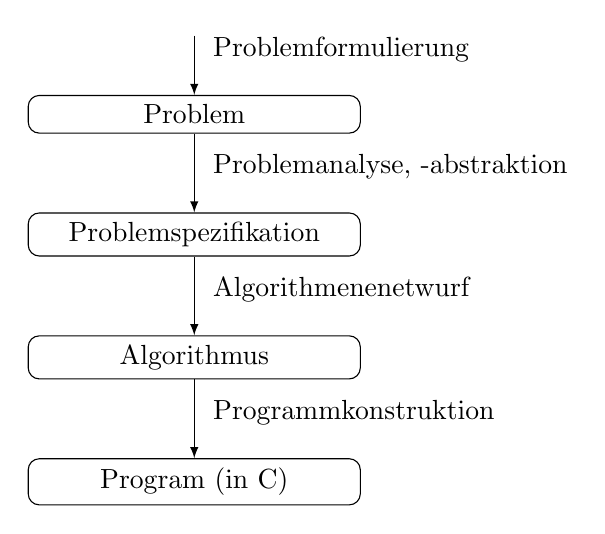
\begin{tikzpicture}
  \node[rounded corners = .4em, draw, minimum width = 12em] at (0, -1) (prob) {Problem};
  \node[rounded corners = .4em, draw, minimum width = 12em, below = of prob] (spez) {Problemspezifikation};
  \node[rounded corners = .4em, draw, minimum width = 12em, below = of spez] (algo) {Algorithmus};
  \node[rounded corners = .4em, draw, minimum width = 12em, below = of algo] (prog) {Program (in C)};

  \node[above right = .3cm and -2cm of prob] {Problemformulierung};
  \node[above right = .3cm and -2cm of spez] {Problemanalyse, -abstraktion};
  \node[above right = .3cm and -2cm of algo] {Algorithmenenetwurf};
  \node[above right = .3cm and -2cm of prog] {Programmkonstruktion};

  \draw[-latex] (0, 0) -> (prob.north);
  \draw[-latex] (prob.south) -> (spez.north);
  \draw[-latex] (spez.south) -> (algo.north);
  \draw[-latex] (algo.south) -> (prog.north);
\end{tikzpicture}

\subsection*{Beispiel}

\subsubsection*{Problemformulierung}

\textbf{Problem}

Suche die jüngste Person im Raum

\subsubsection*{Problemanalyse, -abstraktion}
\begin{itemize}
\item Gibt es überhaupt eine Lösung?
\item Wenn es eine Lösung gibt, gibt es eine eindeutige Lösung?
\item Wie soll eine Lösung aussehen?
\item Wie sollen die Personen bei der Berechnung der Lösung repräsentiert werden?
\item Wie genau soll das Alter einer Person gezählt werden?
\item Was passiert, wenn zwei Personen gleich alt sind?
\end{itemize}

\subsubsection*{Abstraktion}

\begin{enumerate}
\item Jede Person wird durch eine natürliche Zahl $i$ repräsentiert.
\item Als Alter rechnen wir nur das Alter in Jahren; jede Person $i$ hat also ein Alter $a_i$ (positive, ganze Zahl)
\item Die Zahlen $a_1, a_2, \ldots, a_n$ sind bekannt
\item ``Jüngste'' Person ist eine Person $i$, falls für jede Person $j$ gilt: $a_i \leq a_j$
\item Wenn für zwei Personen $i$ und $j$ gilt: $a_i = a_j$, dann wollen wir als Lösung die bzgl. der Folge
  $a_1, a_2, \ldots, a_n$ erste Person mit Alter $a_i$ als Lösung angeben.
\end{enumerate}

\subsubsection*{Problemspezifikation}

\textbf{Gegeben} Folge $a_1, a_2, \ldots, a_n$ von ganzen, positiven Zahlen \\
\textbf{Gesucht} der kleinste Positivindex $j$ mit $a_j = \text{min}\{a_1, \ldots, a_n\}$

\subsubsection*{Algorithmenentwurf}

Ein Algorithmus ist eine (Rechen-)Vorschrift zur Lösung eines Problems.

Ein Algorithmus hat folgende Eigenschaften:

\begin{itemize}
\item muss so präzise formuliert sein, dass er im Prinzip maschinell ausgeführt werden kann
\item ist ein \emph{abstraktes} Objekt
\item ist unabhängig von der Programmiersprache, in der er implementiert werden soll
\item ist unabhängig vom Computertyp oder der verwendeten Rechnertechnologie
\item ist durch einen endlichen Text beschrieben (\emph{Finitheit})
\item läuft in einzelnen, wohldefinierten Schritten ab (\emph{Effektivität})
\item nach Ausführung jedes Schrittes ist eindeutig festgelegt, welcher Schritt als nächster ausgeführt wird
  (\emph{Determiniertheit})
\item kommt bei jeder Eingabe in endlich vielen Schritten zu einem Ende (\emph{Terminiertheit}).
\end{itemize}

\begin{tabular}{r l}
  \hline
  Algorithmus & MinAlter \\
  \hline
  \textbf{Eingabe} & Eine Folge $a_1, \ldots, a_n$ von positiven, ganzen Zahlen \\
  \textbf{Ausgabe} & Der kleinste Positionsindex $a_j$ mit $a_j = \text{min}\{a_1, \ldots, a_n\}$ \\
  \textbf{Verfahren} &
                       \begin{minipage}[t]{\linewidth}
                       Zusätzliche Variablen: $x \text{ (Für das Alter)}, i \text{ (Als Zählvariable)}$;
  \begin{enumerate}
  \item (\emph{Initialisierung}) Setze $j \coloneqq 1, x \coloneqq a_j, i \coloneqq 2$
  \item (\emph{Suchlauf})
    Solange $i \leq n$ gilt, wiederhole: \\
    falls $a_i < x$, setze $j \coloneqq i$ und $x \coloneqq a_j$ \\
    erhöhe $i$ um $1$
  \item Ausgabe von $j$ als Ergebnis
  \end{enumerate}
  \end{minipage}
  \\
  \\
  \hline
\end{tabular}

\subsubsection*{Programmkonstruktion}

\begin{tabularx}{\textwidth}{X X}
  \hline
  anstehende Frage & unsere Antwort \\
  \hline
  Verfügbare Programmiersprachen? & C \\
  Wie kommen die Daten in den Rechner? & Altersangaben müssen eingegeben werden \\
  Durch welche Datenstruktur werden Daten repräsentiert?  & Die Folge $a_1, \ldots, a_n$ der Zahlen wird in einem
                                                            Array (Feld) gespeichert \\
  Wie wird das Ergebnis ausgegeben? & Ausgabe als verständlicher Text \\
  Wie wird das Programm gegliedert? & Die Operation ``Finde Person mit kleinstem Alter'' wird als Funktion beschrieben. \\
  \hline
\end{tabularx}



\end{document}